\section{Плотностная модель Земли и метод Z-фактора}
\subsection{Модель PREM и расчет толщины}
В качестве модели, которая описывает плотность Земли, используется модель PREM (Предварительная эталонная модель Земли, \cite{dziewonskiPREM1981}). Эта простая модель сферически симметричной Земли, не учитывающая особенности рельефа поверхности земли.  Она включает в себя различные свойства Земли: плотность, давление и гравитацию и остальное.  В данной модели вся кора Земли считается однородной.  Плотность в модели PREM можно увидеть на рис.(\ref{PREM})
\begin{figure}[!h]
\centering
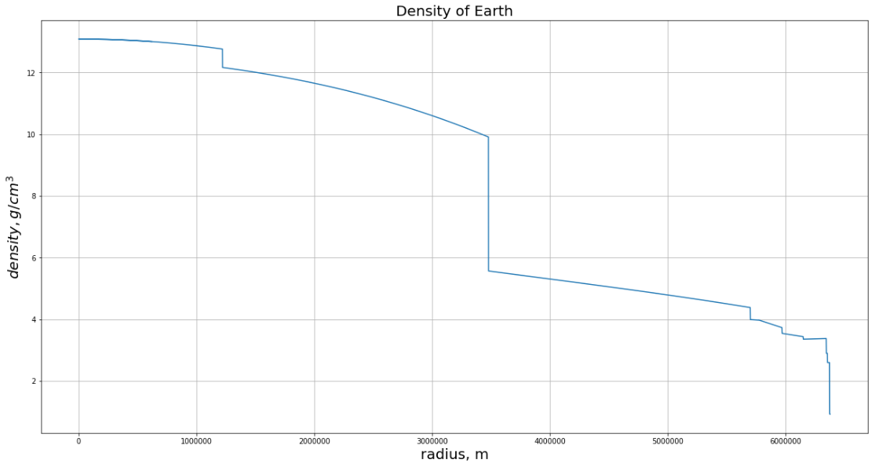
\includegraphics[width=\linewidth]{images/NuProp/PREM.png}
\caption{Плотность вещества в модели Земли PREM.}
\label{PREM}
\end{figure}


Для вычисления переменной $x$ необходимо рассчитать интеграл по траектории нейтрино. Для этих целей используется один из следующих методов: метод прямоугольников (простой метод, дающий хороший результат для функции плотности Земли и работающий быстро для большого количества вызовов функции), метод quad из библиотеки для научных вычислений Scipy (метод, основанный на квадратурных формулах Гаусса) и метод Vegas (Монте-Карло метод, который очень эффективен как для вычисления одномерных, так и для многомерных интегралов). После распространения нейтрино в конечную точку, в ней происходит розыгрыш конечных состояний, в котором учитывается изотопный состав вещества, где происходит взаимодействие. Изотопный состав мишени также задается в модуле Earth нейтринного генератора NuPropagator. 
Данный класс описывает вещество, через которое проходит поток нейтрино. В данной работе рассматривается прохождение нейтрино сквозь Землю, поэтому в дальнейшем будем обсуждать только Землю. Однако, данный генератор может работать абсолютно с любыми плотностями, которые будут поданы в него заранее. 

Учтем, что, проходя сквозь толщу земли, поток нейтрино ослабевает как за счет нейтрального тока, так и за счет заряженного тока. Потери за счет нейтрального тока будут обсуждаться в одном из следующих разделов.
\subsection{Z-фактор: идея и формулы}
Метод Z-фактора помогает нам рассчитать, как изменяются потоки нейтрино при распространении в толщу материи. Опишем его здесь вкратце.  Полное описание можно найти в работе \cite{naumov1999}.

Итак, рассмотрим нейтринный поток $F_{\nu}(x,E)$. Так как за счет заряженного тока нейтрино выбывают из потока, а за счет нейтрального тока они могут изменить энергию и направление, мы можем написать на функцию $F_{\nu}(x,E)$ следующее уравнение
\begin{equation}
\label{eq:Zeq}
    \frac{\partial F_{\nu}(x,E)}{\partial x} = \frac{1}{\lambda_{\nu}(E)}\left[ \int\limits_0^1\frac{dy}{1-y}\Phi_{\nu}(y,E) F_{\nu}(x,E_y) - F_{\nu}(x,E) \right],
\end{equation}
где 
\begin{equation}
    \begin{aligned}
        &x = \int\limits_0^L \rho(L')dL',\\
        &\lambda^{-1}_{\nu}(E) = \sum\limits_{T}N_T\sigma^{tot}_{\nu T}(E),\\
        &\Phi_{\nu}(y,E) = \frac{1}{\lambda_{\nu}(E)}\sum\limits_{T}N_T\frac{d\sigma_{\nu T\to\nu X}}{dy}.
    \end{aligned}
\end{equation}
Здесь $\rho(L)$ — плотность вещества. которая заметается траекторией нейтрино, $N_T$ - число рассеивателей, $E_y = \frac{E}{1-y}$.
Добавим к ур.(\ref{eq:Zeq}) начальное условие, что 
\begin{equation}
    F_{\nu}(x = 0,E) = F^0_{\nu}(E).
\end{equation}

Ищем решение уравнения в следующем виде 
\begin{equation}
    F_{\nu}(x,E) = F^{0}_{\nu}(E)\exp\left(-\frac{x}{\Lambda_{\nu}(x,E)}\right)
\end{equation}
Мы знаем основную асимптотику нашего решения, она имеет вид $\exp\left(-\frac{x}{\Lambda_{\nu}(x,E)}\right)$ (это решение при пренебрежении эффектом изменения энергии нейтрино). Значит, нам надо искать наш фактор в следующем виде:
\begin{equation}
    \Lambda_{\nu}(x,E) = \frac{\lambda_{\nu}(E)}{1 - Z_{\nu}(x,E)}
\end{equation}
Подставляя этот анзатц в уравнение (\ref{eq:Zeq}), получаем уравнение:
\begin{equation}
    Z_{\nu}(x,E) = \int\limits_0^xdx'\int\limits_0^1dy\eta_{\nu}(y,E)\Phi_{\nu}(y,E)\exp\left[ -x'D_{\nu}(x',E,E_y) \right],
\end{equation}
где
\begin{equation}
\label{eq:ZZ2}
\begin{aligned}
    D_{\nu}(x',E,E_y) = & \frac{1 - Z_{\nu}(x,E_y)}{\lambda_{\nu}(E_y)} - \frac{1 - Z_{\nu}(x,E)}{\lambda_{\nu}(E)}\\
    &\eta_{\nu}(y,E) = \frac{F^{0}_{\nu}(E_y)}{F^{0}_{\nu}(E)(1-y)}.\\
\end{aligned}
\end{equation}
К уравнению (\ref{eq:ZZ2}) можно применить итерационную схему
\begin{equation}
    \begin{aligned}
     Z^{(n+1)}_{\nu}(x,E) = &\int\limits_0^xdx'\int\limits_0^1dy\eta_{\nu}(y,E)\Phi_{\nu}(y,E)\exp\left[ -x'D^{(n)}_{\nu}(x',E,E_y) \right],\\
     D^{(n)}_{\nu}(x',E,E_y) =&\frac{1 - Z^{(n)}_{\nu}(x,E_y)}{\lambda_{\nu}(E_y)} - \frac{1 - Z^{(n)}_{\nu}(x,E)}{\lambda_{\nu}(E)}\\
   \end{aligned}
\end{equation}

Наконец, выпишем здесь формулы для первого и второго порядка. 
\begin{equation}
    \begin{aligned}
      Z^{(0)}_{\nu}(x,E) =  &\int\limits_0^1dy\eta_{\nu}(y,E)\Phi_{\nu}(y,E)  = Z_{\nu}(x = 0,E)\\
       Z^{(1)}_{\nu}(x,E) = &\int\limits_0^1dy\eta_{\nu}(y,E)\Phi_{\nu}(y,E)\frac{1 - \exp\left[ -x'A_{\nu}(E,E_y) \right]}{xA_{\nu}(E,E_y)},\\
    \end{aligned}
\end{equation}
где 
\begin{equation}
    A_{\nu}(E,E_y) = \frac{1}{\lambda_{\nu}(E_y)} - \frac{1}{\lambda_{\nu}(E)}
\end{equation}
Физический смысл Z-фактора  - мультипликативная поправка к ослабеванию нейтринного потока при распространении через толщу материи за счет возможных взаимодействий по нейтральному току. Данный метод расчета очень удобен, так как он дает итеративную схему с повышенной сходимостью. Данный метод очень часто используют для задач, где есть кинетические уравнения переноса (в частности, для расчета потоков атмосферных нейтрино \cite{sinegovskaya2015}).
\subsection{Итерационный метод и его реализация в \texttt{NuPropagator}}
Нейтрино может провзаимодействовать в веществе либо с нуклоном, либо с электроном. Если рассматривать заряженный ток, то промежуточным бозоном в данном случае является W-бозон. Значит, в конечном состоянии можно наблюдать лептон и адроны. 
Таким образом, нейтрино, провзаимодействовав в веществе за счет заряженного тока, исчезает (Здесь не рассматривается последующая возможная реакция, описывающая  взаимодействие конечного лептона с нуклоном, в результате которой рождается еще одно нейтрино, так как эта реакция сильно подавлена за счет того, что сечение нейтрино взаимодействия нейтрино с веществом очень мало и по порядку величины равно $10^{-38}$ для 100 ГэВ).
Получается, что за счет заряженного тока поток нейтрино просто ослабевает. Аналогично учитывается и выбывание нейтрино за счет нейтрального тока (Так называемый "эффект регенерации", когда у нейтрино уменьшается энергия за счет нейтрального тока также учитывается, но будет описан позже). 

Соответствующий фактор ослабевания нейтринного потока за счет взаимодействий имеет следующий вид:
\begin{equation}
    \begin{aligned}
            &P(E,x) = \exp(-x/\lambda_{\nu}(E))\\
            &\frac{1}{\lambda_{\nu}(E)} = \sum_TN_T\sigma^{tot}_{vT}(E)\\
            & x = \int\limits_{\gamma}dl\rho(l)
    \end{aligned}
\end{equation}
где $N_T$ — количество рассеивателей на 1 грамм среды типа $T\in \{p,n,e\}$ , $\sigma^{tot}_{vT}(E)$ - полное сечение рассеяния для взаимодействия $\nu T$ и сумма берется по всем возможным типам рассеивающих частиц. Переменная $x$, определяемая как интеграл по траектории нейтрино от плотности вещества, есть толща вещества, которую проходит нейтрино (т.е. длина пути нейтрино в массовых единицах).  
